%%% Template originaly created by Karol Kozioł (mail@karol-koziol.net) and modified for ShareLaTeX use

\documentclass[a4paper,11pt]{article}

\usepackage[T1]{fontenc}
\usepackage[utf8]{inputenc}
\usepackage{graphicx}
\usepackage{xcolor}
 \usepackage{tgtermes}
\usepackage{listings}
\usepackage{minted}
 \usepackage[
 pdftitle={Math Assignment},
 pdfauthor={Joe Doe, Some University},
 colorlinks=true,linkcolor=blue,urlcolor=blue,citecolor=blue,bookmarks=true,
 bookmarksopenlevel=2]{hyperref}
\usepackage{amsmath,amssymb,amsthm,textcomp}
\usepackage{enumerate}
\usepackage{multicol}
\usepackage{tikz}

\usepackage{geometry}
\geometry{total={210mm,297mm},
left=25mm,right=25mm,%
bindingoffset=0mm, top=20mm,bottom=20mm}


\linespread{1.3}

\newcommand{\linia}{\rule{\linewidth}{0.5pt}}

% custom theorems if needed
\newtheoremstyle{mytheor}
    {1ex}{1ex}{\normalfont}{0pt}{\scshape}{.}{1ex}
    {{\thmname{#1 }}{\thmnumber{#2}}{\thmnote{ (#3)}}}

\theoremstyle{mytheor}
\newtheorem{defi}{Definition}
\usepackage[ruled, vlined, linesnumbered,lined,boxed,commentsnumbered]{algorithm2e}
\usepackage[parfill]{parskip}
\makeatletter

\setlength\parindent{0pt}
% custom footers and headers
\usepackage{fancyhdr,lastpage}


\newcommand{\myequ}[1]{\begin{align}\begin{split} #1 \end{split}\end{align}}


\begin{document}

\title{CSE 250B: Machine Learning}

\author{Sai Bi}

\date{\today}

\maketitle

\section*{Problem 1}
\subsection*{a}
See Figure~\ref{fig:1a}. The decision boundary is not linear.
\begin{figure}[b]
	\centering{
		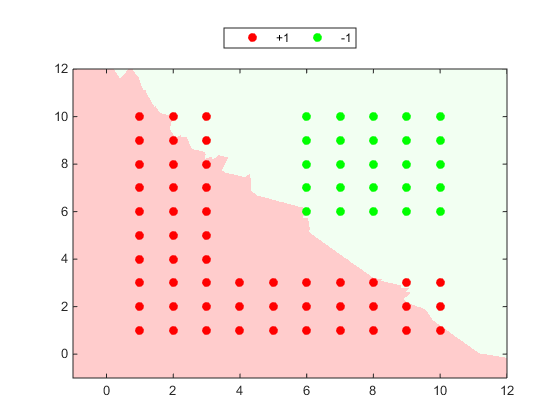
\includegraphics[width = 0.9\textwidth]{./code/1a.png}
	}
	\caption{Problem 1-a, $T = 10$}
	\label{fig:1a}
\end{figure}

\subsection*{b}
See Figure~\ref{fig:1b}.

\begin{minted}[frame=lines, framesep=2mm,]
{cpp}
Input: T, x, y, L
l = 1, c = 0
w = 0
heap = make_min_heap()
flag = false
Repeat T times
	Randomly permute the data points
	for i = 1 to n:
		if (x_i, y_i) is misclassified by w:
			insert (c, w) into heap
			if heap.size() > L
				heap.pop_heap()
				
			w = w + y_i * x_i
			c = 1
			flag = false
		else
			c = c + 1
			flag = true

if flag == true
	insert (c, w) into heap
	if heap.size() > L
		heap.pop_heap() 

return all (w, c) that is in the heap
\end{minted}

\begin{figure}[b]
	\centering{
		\includegraphics[width = 0.45\textwidth]{./code/1b-full.png}
		\includegraphics[width = 0.45\textwidth]{./code/1b-select.png}
	}
	\caption{Problem 1-b. Left: use all $869$ $w$ got in vote perceptron for prediction. 
		Right: use only $L = 50$ for prediction.}
	\label{fig:1b}
\end{figure}

\subsection*{c}
See Figure~\ref{fig:1c}.
\begin{minted}[frame=lines, framesep=2mm,]
{cpp}
Input: T, x, y
c = 0
w = 0
curr_w = 0
flag = false
Repeat T times
	Randomly permute the data points
	for i = 1 to n:
		if (x_i, y_i) is misclassified by w_l:
			w = w + curr_w * c
			curr_w = curr_w + y_i * x_i
			c = 1
			flag = false
		else
			c = c + 1
			flag = true
if flag == true
	w = w + curr_w * c

return w
\end{minted}


\begin{figure}[b]
	\centering{
		\includegraphics[width = 0.9\textwidth]{./code/1c.png}
	}
	\caption{Problem 1-c, $T = 10$}
	\label{fig:1c}
\end{figure}

\section*{Problem 2}
See Figure~\ref{fig:2a-2}, \ref{fig:2a-3}, \ref{fig:2a-4}, \ref{fig:2a-5}.

\begin{figure}[b]
	\centering{
		\includegraphics[width = 0.9\textwidth]{./code/2a-data-1.png}
	}
	\caption{Problem 2. Decision boundary of data1.txt with quadratic kernel. $T = 10000$.}
	\label{fig:2a-2}
\end{figure}

\begin{figure}[b]
	\centering{
		\includegraphics[width = 0.9\textwidth]{./code/2a-data-2.png}
	}
	\caption{Problem 2. Decision boundary of data2.txt with quadratic kernel. $T = 10000$.}
	\label{fig:2a-3}
\end{figure}

\begin{figure}[b]
	\centering{
		\includegraphics[width = 0.45\textwidth]{./code/2-rbf-data-1-sigma-0_5.png}
		\includegraphics[width = 0.45\textwidth]{./code/2-rbf-data-1-sigma-1.png}
		\includegraphics[width = 0.45\textwidth]{./code/2-rbf-data-1-sigma-1_5.png}
		\includegraphics[width = 0.45\textwidth]{./code/2-rbf-data-1-sigma-2.png}
	}
	\caption{Problem 2. Decision boundary of data1.txt with RBF kernel.}
	\label{fig:2a-4}
\end{figure}


\begin{figure}[b]
	\centering{
		\includegraphics[width = 0.45\textwidth]{./code/2-rbf-data-2-sigma-0_5.png}
		\includegraphics[width = 0.45\textwidth]{./code/2-rbf-data-2-sigma-1.png}
		\includegraphics[width = 0.45\textwidth]{./code/2-rbf-data-2-sigma-1_5.png}
		\includegraphics[width = 0.45\textwidth]{./code/2-rbf-data-2-sigma-2.png}
	}
	\caption{Problem 2. Decision boundary of data2.txt with RBF kernel.}
	\label{fig:2a-5}
\end{figure}








\end{document}
